%% Copernicus Publications Manuscript Preparation Template for LaTeX Submissions
%% ---------------------------------
%% This template should be used for copernicus.cls
%% The class file and some style files are bundled in the Copernicus Latex Package, which can be downloaded from the different journal webpages.
%% For further assistance please contact Copernicus Publications at: production@copernicus.org
%% https://publications.copernicus.org/for_authors/manuscript_preparation.html

%% copernicus_rticles_template (flag for rticles template detection - do not remove!)

%% Please use the following documentclass and journal abbreviations for discussion papers and final revised papers.

%% 2-column papers and discussion papers
\documentclass[essd, manuscript]{copernicus}



%% Journal abbreviations (please use the same for preprints and final revised papers)

% Advances in Geosciences (adgeo)
% Advances in Radio Science (ars)
% Advances in Science and Research (asr)
% Advances in Statistical Climatology, Meteorology and Oceanography (ascmo)
% Annales Geophysicae (angeo)
% Archives Animal Breeding (aab)
% Atmospheric Chemistry and Physics (acp)
% Atmospheric Measurement Techniques (amt)
% Biogeosciences (bg)
% Climate of the Past (cp)
% DEUQUA Special Publications (deuquasp)
% Drinking Water Engineering and Science (dwes)
% Earth Surface Dynamics (esurf)
% Earth System Dynamics (esd)
% Earth System Science Data (essd)
% E&G Quaternary Science Journal (egqsj)
% EGUsphere (egusphere) | This is only for EGUsphere preprints submitted without relation to an EGU journal.
% European Journal of Mineralogy (ejm)
% Fossil Record (fr)
% Geochronology (gchron)
% Geographica Helvetica (gh)
% Geoscience Communication (gc)
% Geoscientific Instrumentation, Methods and Data Systems (gi)
% Geoscientific Model Development (gmd)
% History of Geo- and Space Sciences (hgss)
% Hydrology and Earth System Sciences (hess)
% Journal of Bone and Joint Infection (jbji)
% Journal of Micropalaeontology (jm)
% Journal of Sensors and Sensor Systems (jsss)
% Magnetic Resonance (mr)
% Mechanical Sciences (ms)
% Natural Hazards and Earth System Sciences (nhess)
% Nonlinear Processes in Geophysics (npg)
% Ocean Science (os)
% Polarforschung - Journal of the German Society for Polar Research (polf)
% Primate Biology (pb)
% Proceedings of the International Association of Hydrological Sciences (piahs)
% Safety of Nuclear Waste Disposal (sand)
% Scientific Drilling (sd)
% SOIL (soil)
% Solid Earth (se)
% The Cryosphere (tc)
% Weather and Climate Dynamics (wcd)
% Web Ecology (we)
% Wind Energy Science (wes)

% Pandoc citation processing

% The "Technical instructions for LaTex" by Copernicus require _not_ to insert any additional packages.
% % % From pandoc table feature
% \usepackage{longtable,booktabs,array}
% % \usepackage{calc} % for calculating minipage widths
% % Correct order of tables after \paragraph or \subparagraph
% \usepackage{etoolbox}
% \makeatletter
% \patchcmd\longtable{\par}{\if@noskipsec\mbox{}\fi\par}{}{}
% \makeatother
% % Allow footnotes in longtable head/foot
% \IfFileExists{footnotehyper.sty}{\usepackage{footnotehyper}}{\usepackage{footnote}}
% \makesavenoteenv{longtable}
% 
% tightlist command for lists without linebreak
\providecommand{\tightlist}{%
  \setlength{\itemsep}{0pt}\setlength{\parskip}{0pt}}


%
\begin{document}


\title{Transition from forest to agriculture in the Brazilian Amazon from 1985 to 2021}


\Author[1, 2]{Hugo}{Tameirão Seixas}
\Author[2]{Hilton}{Luis Ferraz da Silveira}
\Author[2]{Alan}{Falcão}
\Author[2]{Fabiana}{Da Silva Soares}
\Author[1]{Ramon}{Bicudo}


\affil[1]{Center for Environmental Studies and Research, University of Campinas, Rua dos Flamboyants 155, Brazil}
\affil[2]{Embrapa Territorial, Av. Soldado Passarinho 303, Brazil}

\runningtitle{Transition from forest to agriculture in the Brazilian Amazon from 1985 to 2021}

\runningauthor{Seixas et al.}


\correspondence{Hugo\ Tameirão Seixas\ (seixas.hugo@protonmail.com)}



\received{}
\pubdiscuss{} %% only important for two-stage journals
\revised{}
\accepted{}
\published{}

%% These dates will be inserted by Copernicus Publications during the typesetting process.


\firstpage{1}

\maketitle


\begin{abstract}
A new dataset was created by calculating the time necessary for deforested forests to transition to agriculture in the Brazillian Amazon biome. The new data can be useful in interdiciplinary studies about land cover and land use change in brazil, its drivers and implications. A main inovation is that the dataset links the deforestation year with the year of agriculture establishment, which can provide new information about this process.
\end{abstract}


\copyrightstatement{The author's copyright for this publication is transferred to institution/company.}


\introduction[Introduction]

In the last decades, the Amazon biome have been submitted to strong changes, the advance of agricultural areas over native forests is shaping a new landscape in the region.
The most common pattern of transitions from natural forest formations to agriculture sites, is the initial process of deforestation, followed by the establishment of pasture, where extensive livestock production takes place, until its replacement to agricultural activities.
This process can take several decades to be accomplished, or even less than one year, in which it may be considered as a direct transition from forest to agriculture.

Land cover transitions can cause important impacts on ecosystem properties \citep{Nunes2022}.

This project aims to characterize and quantify the length of the transitions from forest formations to agriculture in the Amazon.

\section{Methods}

The estimations of transition from forest to agriculture were performed for the Amazon biome region, as defined by the Brazilian Institute of Geography and Statistics (IBGE), in 2019.
Transitions were calculated using land use and land cover classification data from MapBiomas \citep{Souza2020}, which ranges from 1985 to 2021, at a spatial resolution of approximately 30 meters.
The data was filtered to contain only pixels that were occupied by forest and agriculture at some period, and that are not considered as water, according to the Global Surface Water product provided by Copernicus \citep{Pekel2016}.

Transition length was calculated pixel by pixel, by performing the following steps:

\begin{enumerate}
\def\labelenumi{\arabic{enumi}.}
\item
  Load raster and extract valid values into a table;
\item
  Calculate the year of first occurrence of a non-natural LULC class for each pixel;
\item
  Calculate the first year of ``Forest Formation'' LULC class after the year calculated in step 2;
\item
  Classify rows as ``before'' or ``after'' the occurrence of the year calculated in step 3;
\item
  Calculate the last year of ``Forest Formation'' within the rows classified as ``before'', and add 1 year to represent the deforestation year;
\item
  Calculate the first year of any agriculture type class within the rows classified as ``before'', for each pixel;
\item
  Calculate the difference between years from items 5 and 6 to get the LULC transition length in years, for each pixel;
\end{enumerate}

The steps 2 to 7 are performed recursively to identify multiple transitions, in case they are present.
Because of the amount of data, the processing and storage was performed in batches of data, structured in raster tiles.

\section{Description of data collection}

After the calculation of transitions, the results are stored in three different types of tables, organized in a folder structure and stored as Apache Parquet files.

\begin{itemize}
\item
  Tables that contains the spatial information (longitude, latitude) of each pixel, its unique id and the code of the municipality which contains the pixel.
  It is named as ``mask\_cells'';
\item
  Tables with transition length values, the first and last year of the transition, the resulting agriculture type, and the number of the transition cycle.
  They also contain the unique id of each pixel (related to the table above);
\item
  Table with the LULC classes of all years within the transition, and also the first 5 years after the transition.
\end{itemize}

The three tables are related to each other and can be used altogether, and are separated by tiles.
Another table containing the metadata of each tile is also created, and holds the spatial characteristics of the tiles.
With this spatial information, it is possible to convert the tabular data back to spatial raster, with identical spatial properties as the MapBiomas classification data.

\section{Results and discussion}

The transition calculations shows that between 1985 and 2021, 64874 squared kilometers of forests were converted to agriculture, in the Brazilian Amazon biome.
The length of the transitions can go from 1 to 36 years, in which transitions closer to 1 year are considered as fast transitions, and transitions closer to 36 years are considered as slow transitions.
Transitions of 1 year are considered as ``direct'' transitions, where there were no presence of pasture before the establishment of agriculture, out estimations shows that around 9.2 \% of the transitions are considered as ``direct''.

Although we named as deforestation the last years identified as forest before classification of anthropic cover, we acknowledge that it is not a direct measurement of deforestation (such as PRODES), it is however a proxy to deforestation.

\subsection{Transition patterns}

Transitions from forest to agriculture can be found in almost every region in the Amazon, but is mostly concentrated in clusters, specially in the south and east of the biome, in the states of Mato Grosso, Pará and Maranhão (Figure \ref{fig:map-plot}).

\begin{figure}[ht]
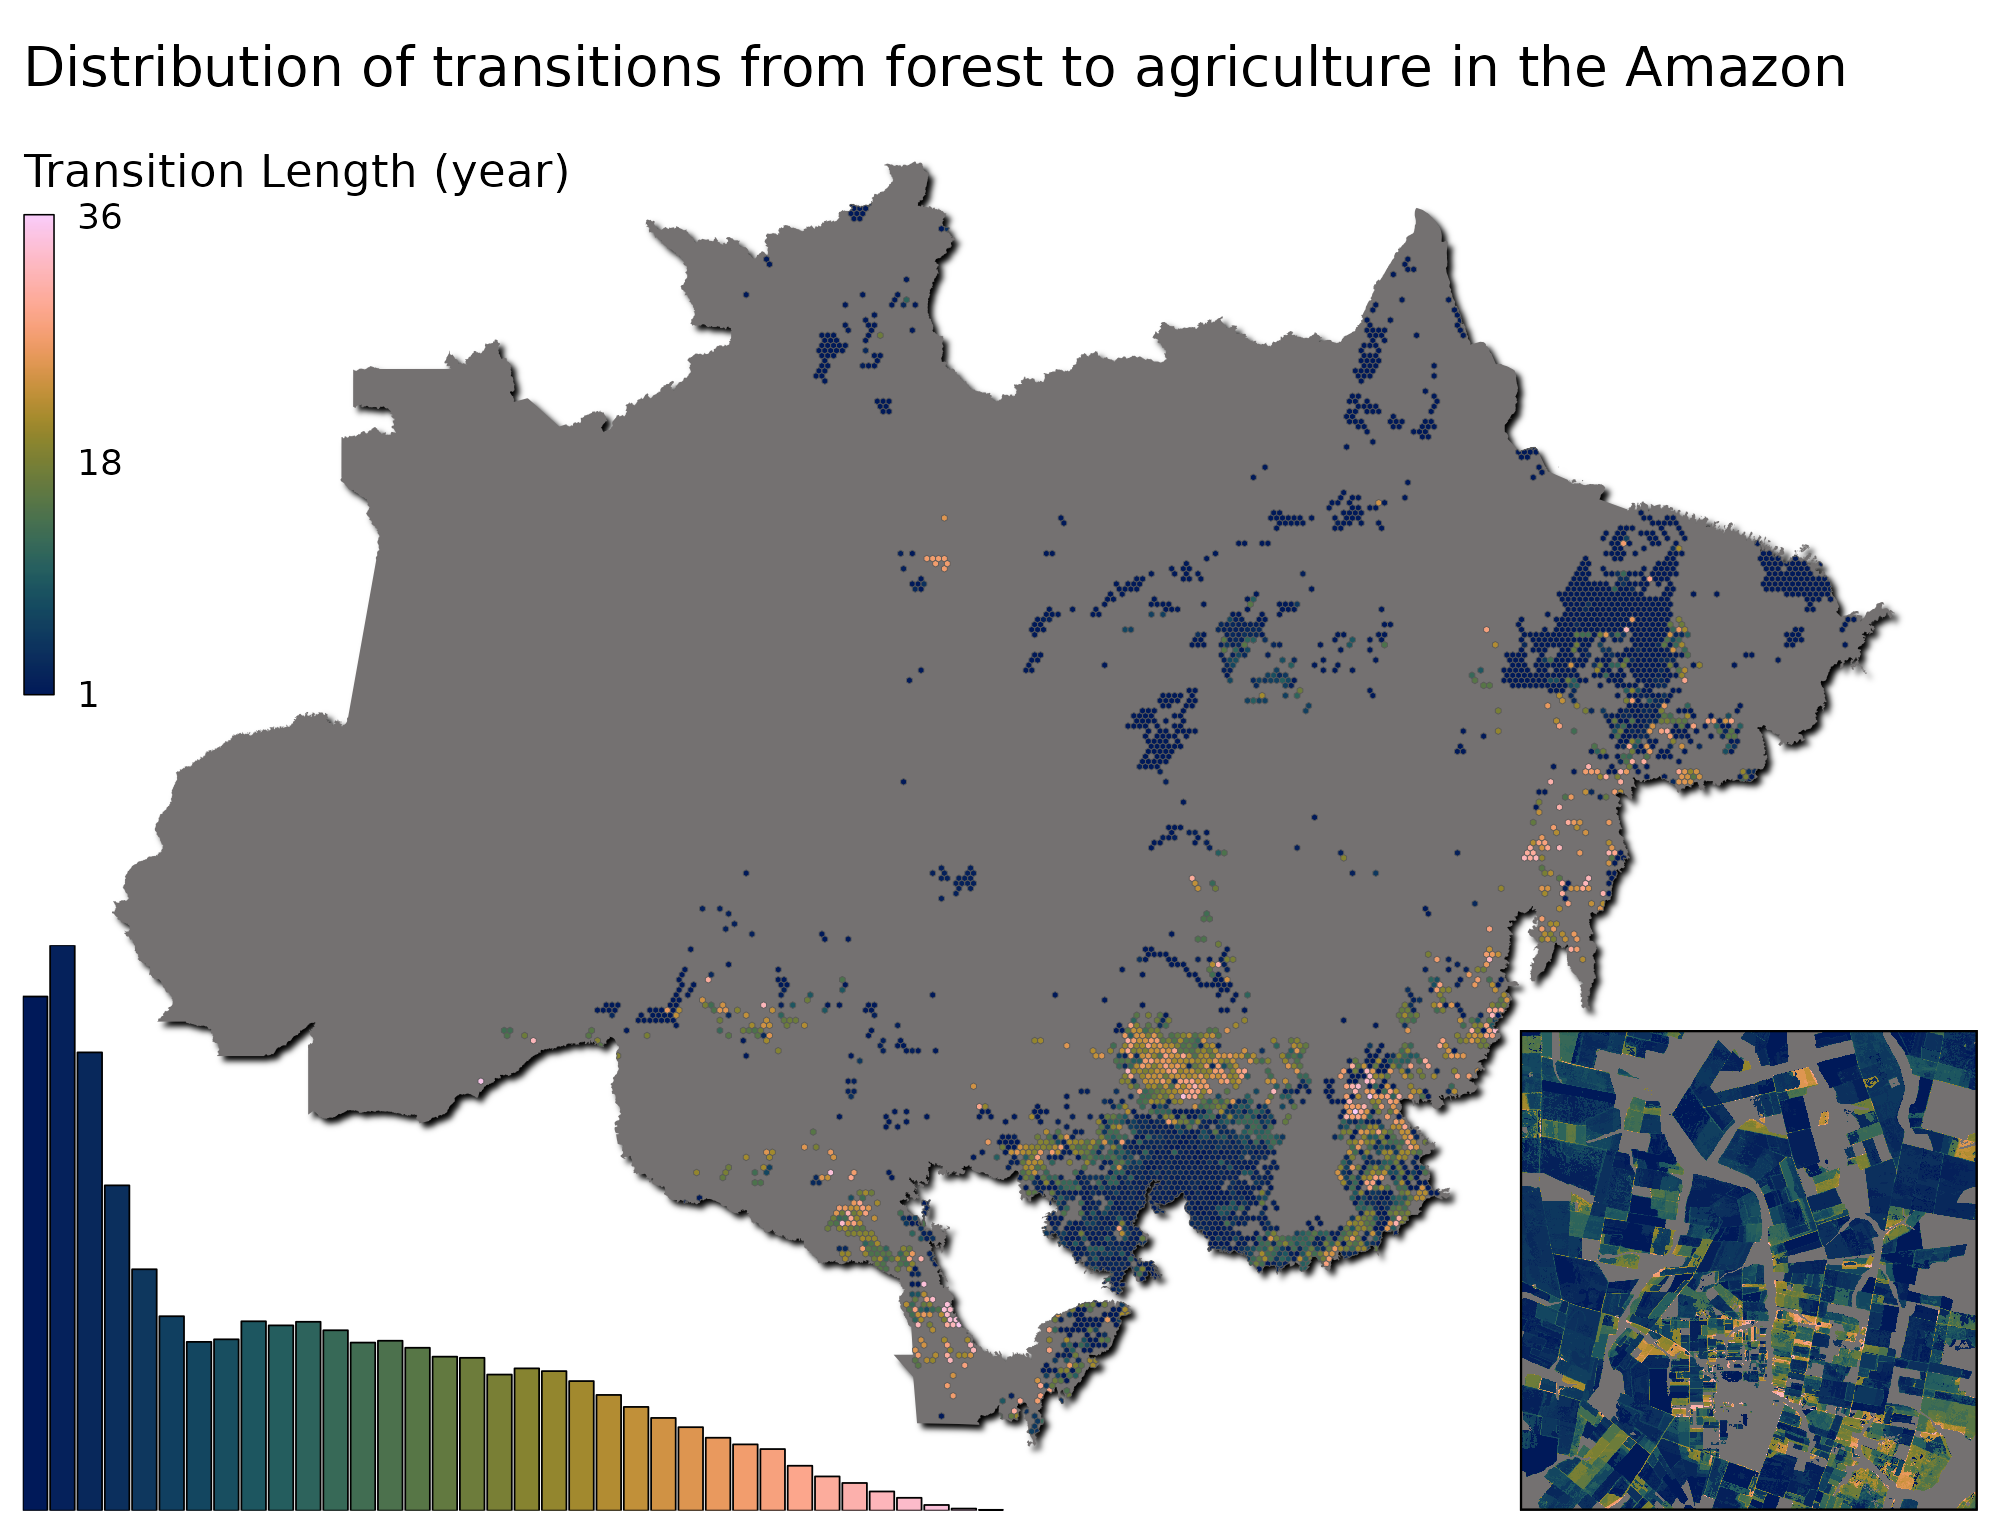
\includegraphics[width=17cm]{figs/map} \caption{Map of distribution of transitions from forests to agriculture in the Brazillian Amazon biome. The hexagonal cells represent the most common transition length, and do not reflect the amount of area of transitions inside a cell. Transitions are concentraded in the south (Mato Grosso state), and in the east (Pará and Maranhão states). The transition length ranges from 1 (blue tones) to 36 years (pink tones), and clusters of fast transitions (transitions closer to 1 year) can be discerned from clusters of slow transitions (transitions closer to 36 years). The histogram located in the bottom left shows that fast transitions are more common than slower transitions. The zoomed map in the bottom right shows the results in finer resolution, where it is possible to observe different transition lengths between properties.}\label{fig:map-plot}
\end{figure}

Well defined clusters can be observed in the map created with aggregated transition length data (Figure \ref{fig:map-plot}), slow transition areas tend to concentrate in specific regions in the Amazon biome, while fast transitions seem to have a wider distributions, but also tend to form clusters.
However, this pattern does not hold completely when observing the data at its original scale (Figure \ref{fig:map-plot}), where areas with different transition lengths are mixed between each other.
When observing at the original scale, we could not spot any well defined pattern or direction of the occurrence of faster to slower transitions (Figure \ref{fig:map-plot}).

Other studies investigating patterns of transitions in the Amazon also found the formation of clusters of patterns, although there is a big heterogeneity at larger scales \citep{MullerHansen2017}.

The data can be analysed year by year, and also be separated by primary and secondary forests being converted to agriculture (Figure \ref{fig:transbar-plot}).

\begin{figure}[ht]
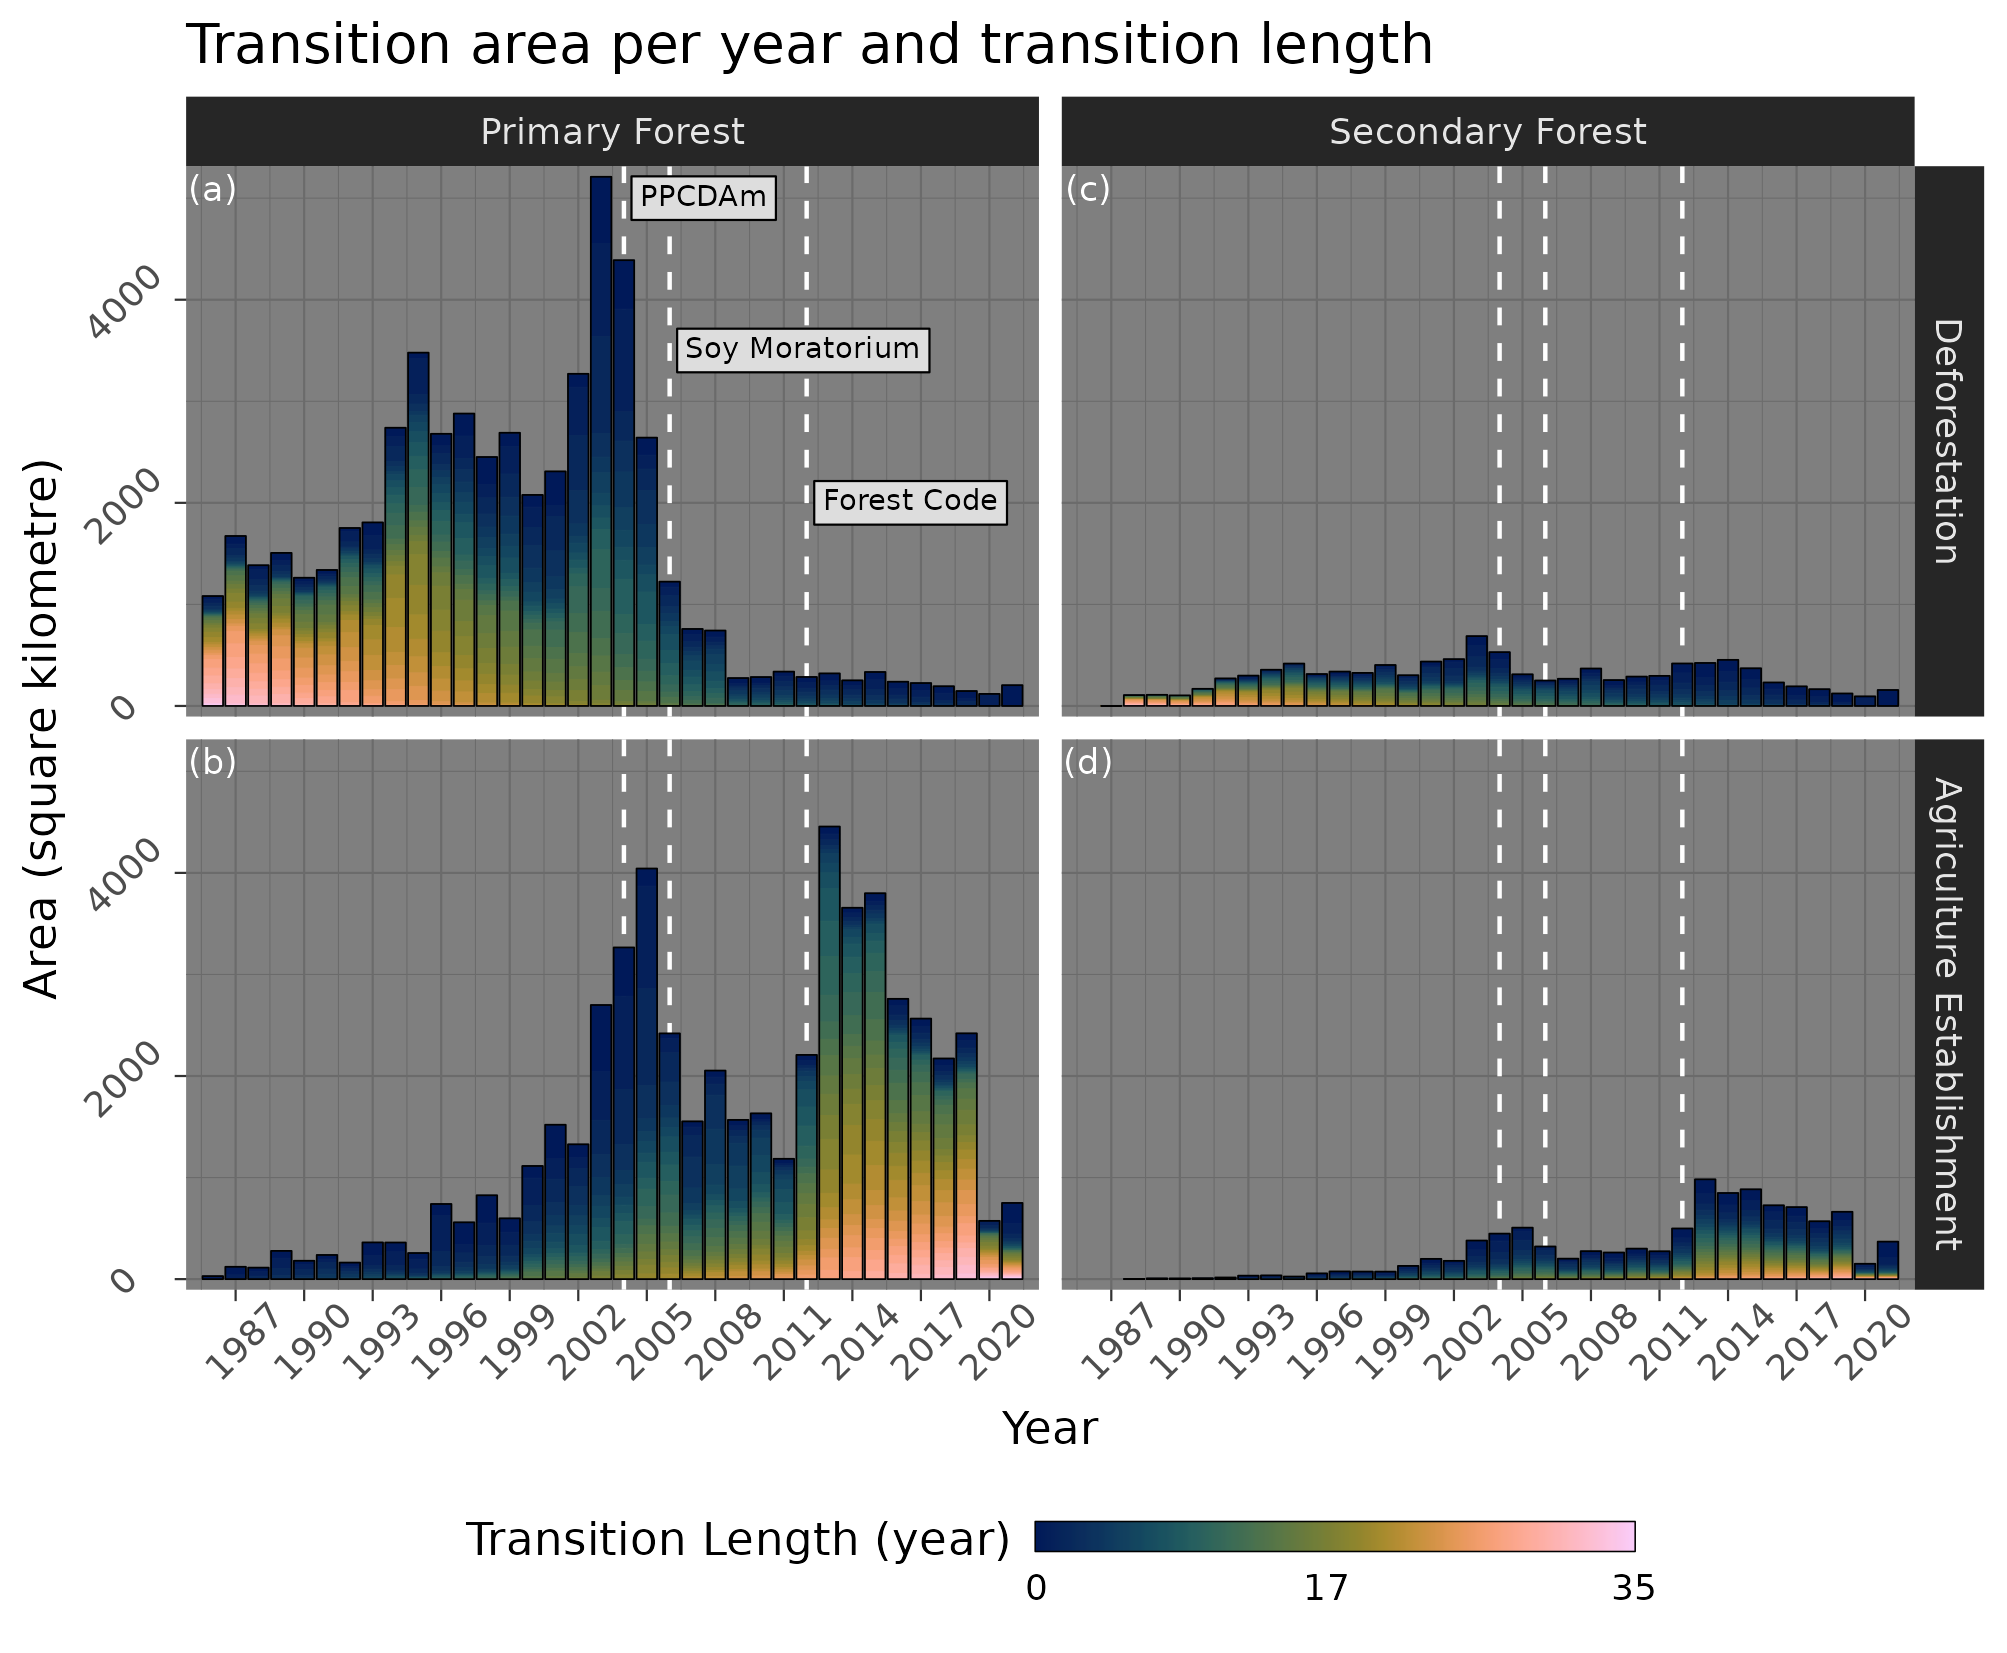
\includegraphics[width=17cm]{figs/trans_length_cols} \caption{Transition area per year and transition length. The bars represent the total amount of area at some state of the transition for each year. The color gradient in each bar represents the transition length related to a deforestation or a agriculture establishment event. Blue tones represents fast transitions (transitions closer to 0 years), pink tones represents slow transitions (transitions closer to 35 years). Transition events were separated by deforestation of primary forests (a) and secondary forests (c), and the subsequent  agriculture establishment of primary forests (b) and secondary forests (d).}\label{fig:transbar-plot}
\end{figure}

The deforestation area of primary forests increased largely from 1986 to 2003, which was followed be a steep decrease until 2009, when the deforested areas reached a stable rate.
From 1986 to approximately 1995, most of deforested areas suffered a slow transition, mostly were higher than 10 years, after this period, fast transitions started to become more common, specially from 2002 to 2004.

Agriculture establishment over areas of primary forests peaked in 2005 and 2013.
Despite similar rates between both years, their transition lengths differ greatly, in 2005 most of the transitions were faster than 10 years, while in 2013 the great majority of transitions were slower than 10 years.
The year of 2003 marked a change in the transition length of establishment of agriculture areas, after this year, most of the transitions happened in areas deforested at least 10 years before.
Even after the decrease of deforestation after 2002, agriculture areas are expanding over lands where deforestation happened before 2002.
However, after 2019, a sudden drop of agriculture establishment rate happened.

The causes of deforestation and agriculture establishment in the Brazilian Amazon are complex and diverse.
Political context, public policies, market prices and law enforcement can influence how these processes evolve over time.
In 2004, the Brazilian Government launched the Action Plan for the Prevention and Control of Deforestation in the Legal Amazon (PPCDAm), which was composed by many initiatives to curb deforestation \citep{West2021}.
The PPCDAm was considered as a successful policy to slow deforestation rates in Brazil, with international recognition.
Our calculations from MapBiomas data reinforces the corelation of the PPCDAm with the reduction of deforestation after 2004, and reduction of the agriculture establishment after 2005.

In 2006, the Brazilian Association of Vegetable Oil Industries (BIOVE) and the National Association of Cereal Exporters (ANEC) committed to avoid commercialization of soy grains harvested from areas deforested after 2006.
Our estimates of transitions show a decrease of deforested areas to be converted to agriculture after 2008, where it reached minimal values (Figure \ref{fig:transbar-plot}.a).
After 2006, agriculture establishment over deforested primary forests suffered a decrease, which stayed relatively stable until 2012, where a steep increase occurred, however, the new areas being occupied by agriculture were mainly over areas that were cleared more than a decade before (therefore, before 2006) (Figure \ref{fig:transbar-plot}.b) This shows that agriculture expansion did not halt after the soy moratorium, producers started expanding in old cleared areas.
Expansion of agriculture areas also expanded over cleared areas of secondary forests in 2012, but with an important amount of fast transitions.
The causes of the increase of agriculture establishment areas can be numerous, one main driver was the approval of a new Forest Code, in 2012, which is considered to have undermined the environmental protection of forests \citep{Kroger2017, Pereira2019}.

The transition length patterns across years can change significantly between different states (Figure \ref{fig:transridge-plot}).

\begin{figure}[ht]
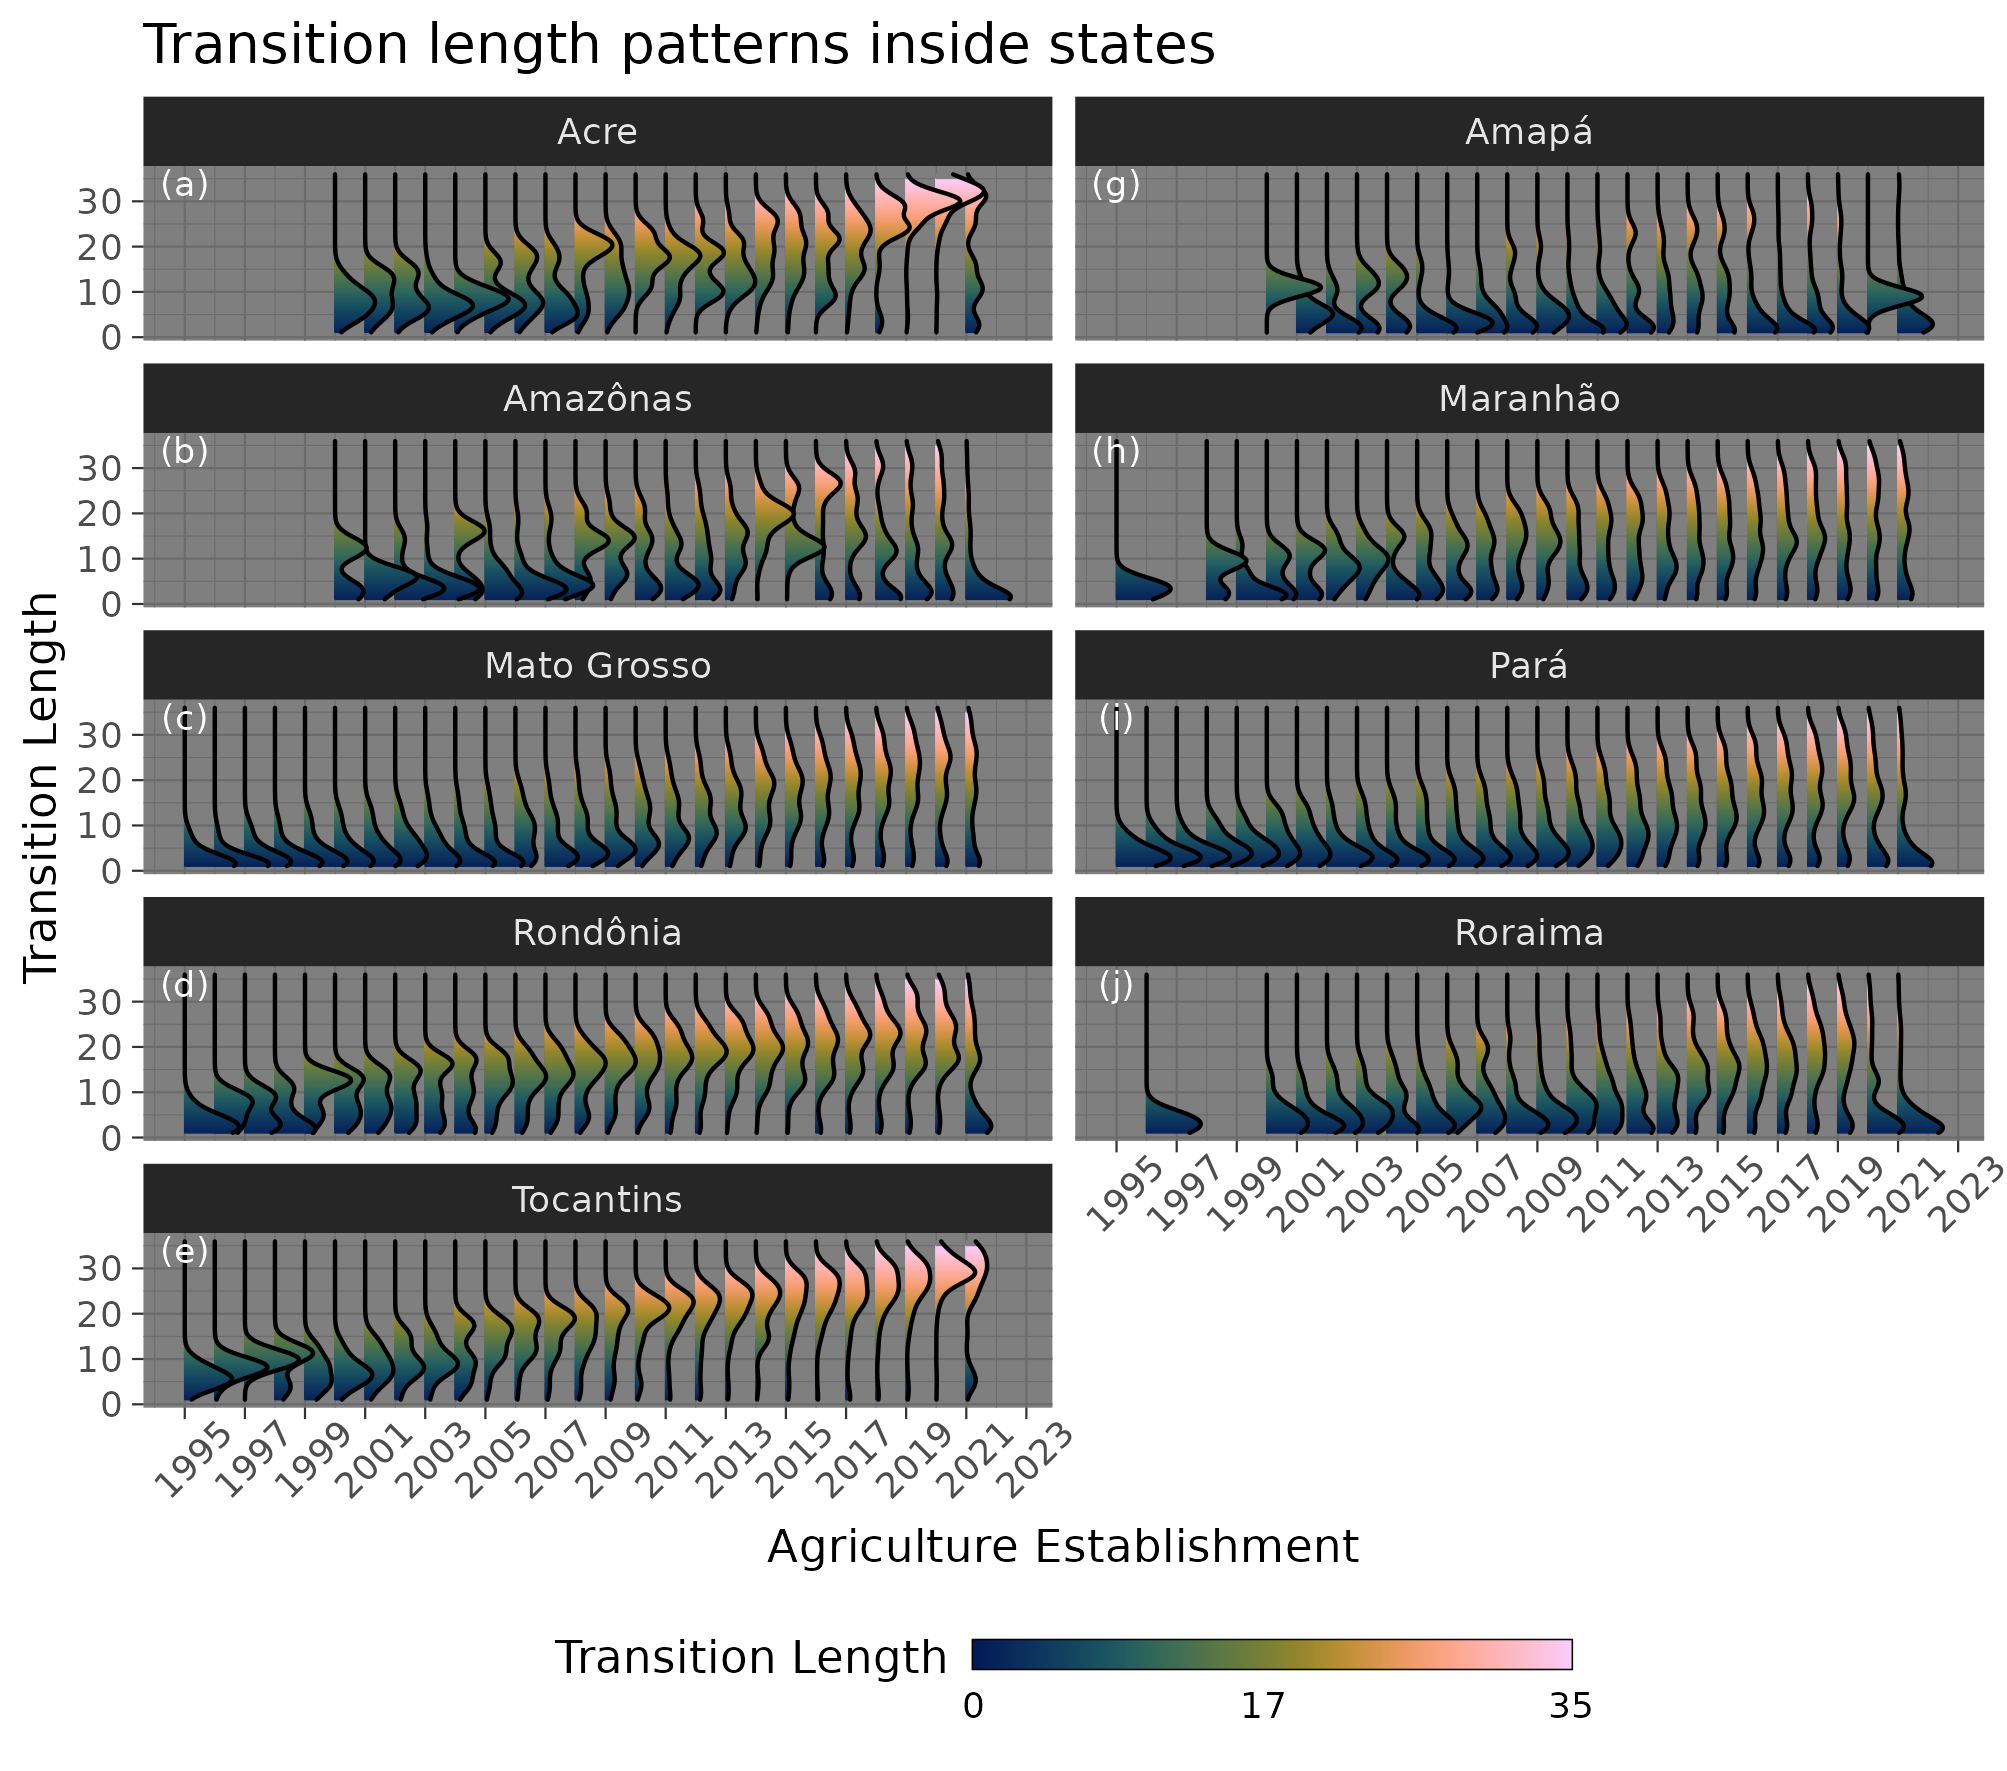
\includegraphics[width=17cm]{figs/trans_ridge} \caption{Transition length patterns inside states that belongs to the Amazon biome. Each year have a density estimate of the transition lengths, represented as colored curves. The peak of the curves represents transition length values with more frequency in one year of one state. Blue tones represents fast transitions (transitions closer to 0 years), pink tones represents slow transitions (transitions closer to 35 years)}\label{fig:transridge-plot}
\end{figure}

The state of Amapá presented fast transitions along all the time series, where slow transitions are not as common.
In contrast, Acre shows a majority of slow transitions, in which only 2021 showed more fast transitions.
There are three states where the pattern of transitions length across time are alike, Mato Grosso, Pará and Rondônia presented more fast transitions from 1995 to 2005, after this period, slow transitions became more common with time, until around 2015, where the occurrence of fast transitions were the majority again.

\subsection{Validation}

When analyzing the errors from the transition length estimates, we observe that the year of deforestation shows the least amount of errors (Figure \ref{fig:errorbar-plot}).
The MAE of the deforestation year is of 1.42 years, and the error shows a bias towards underestimation.
The year of the agriculture establishment and the transition length estimates showed larger errors when comparing with visual inspection.

\begin{figure}[ht]
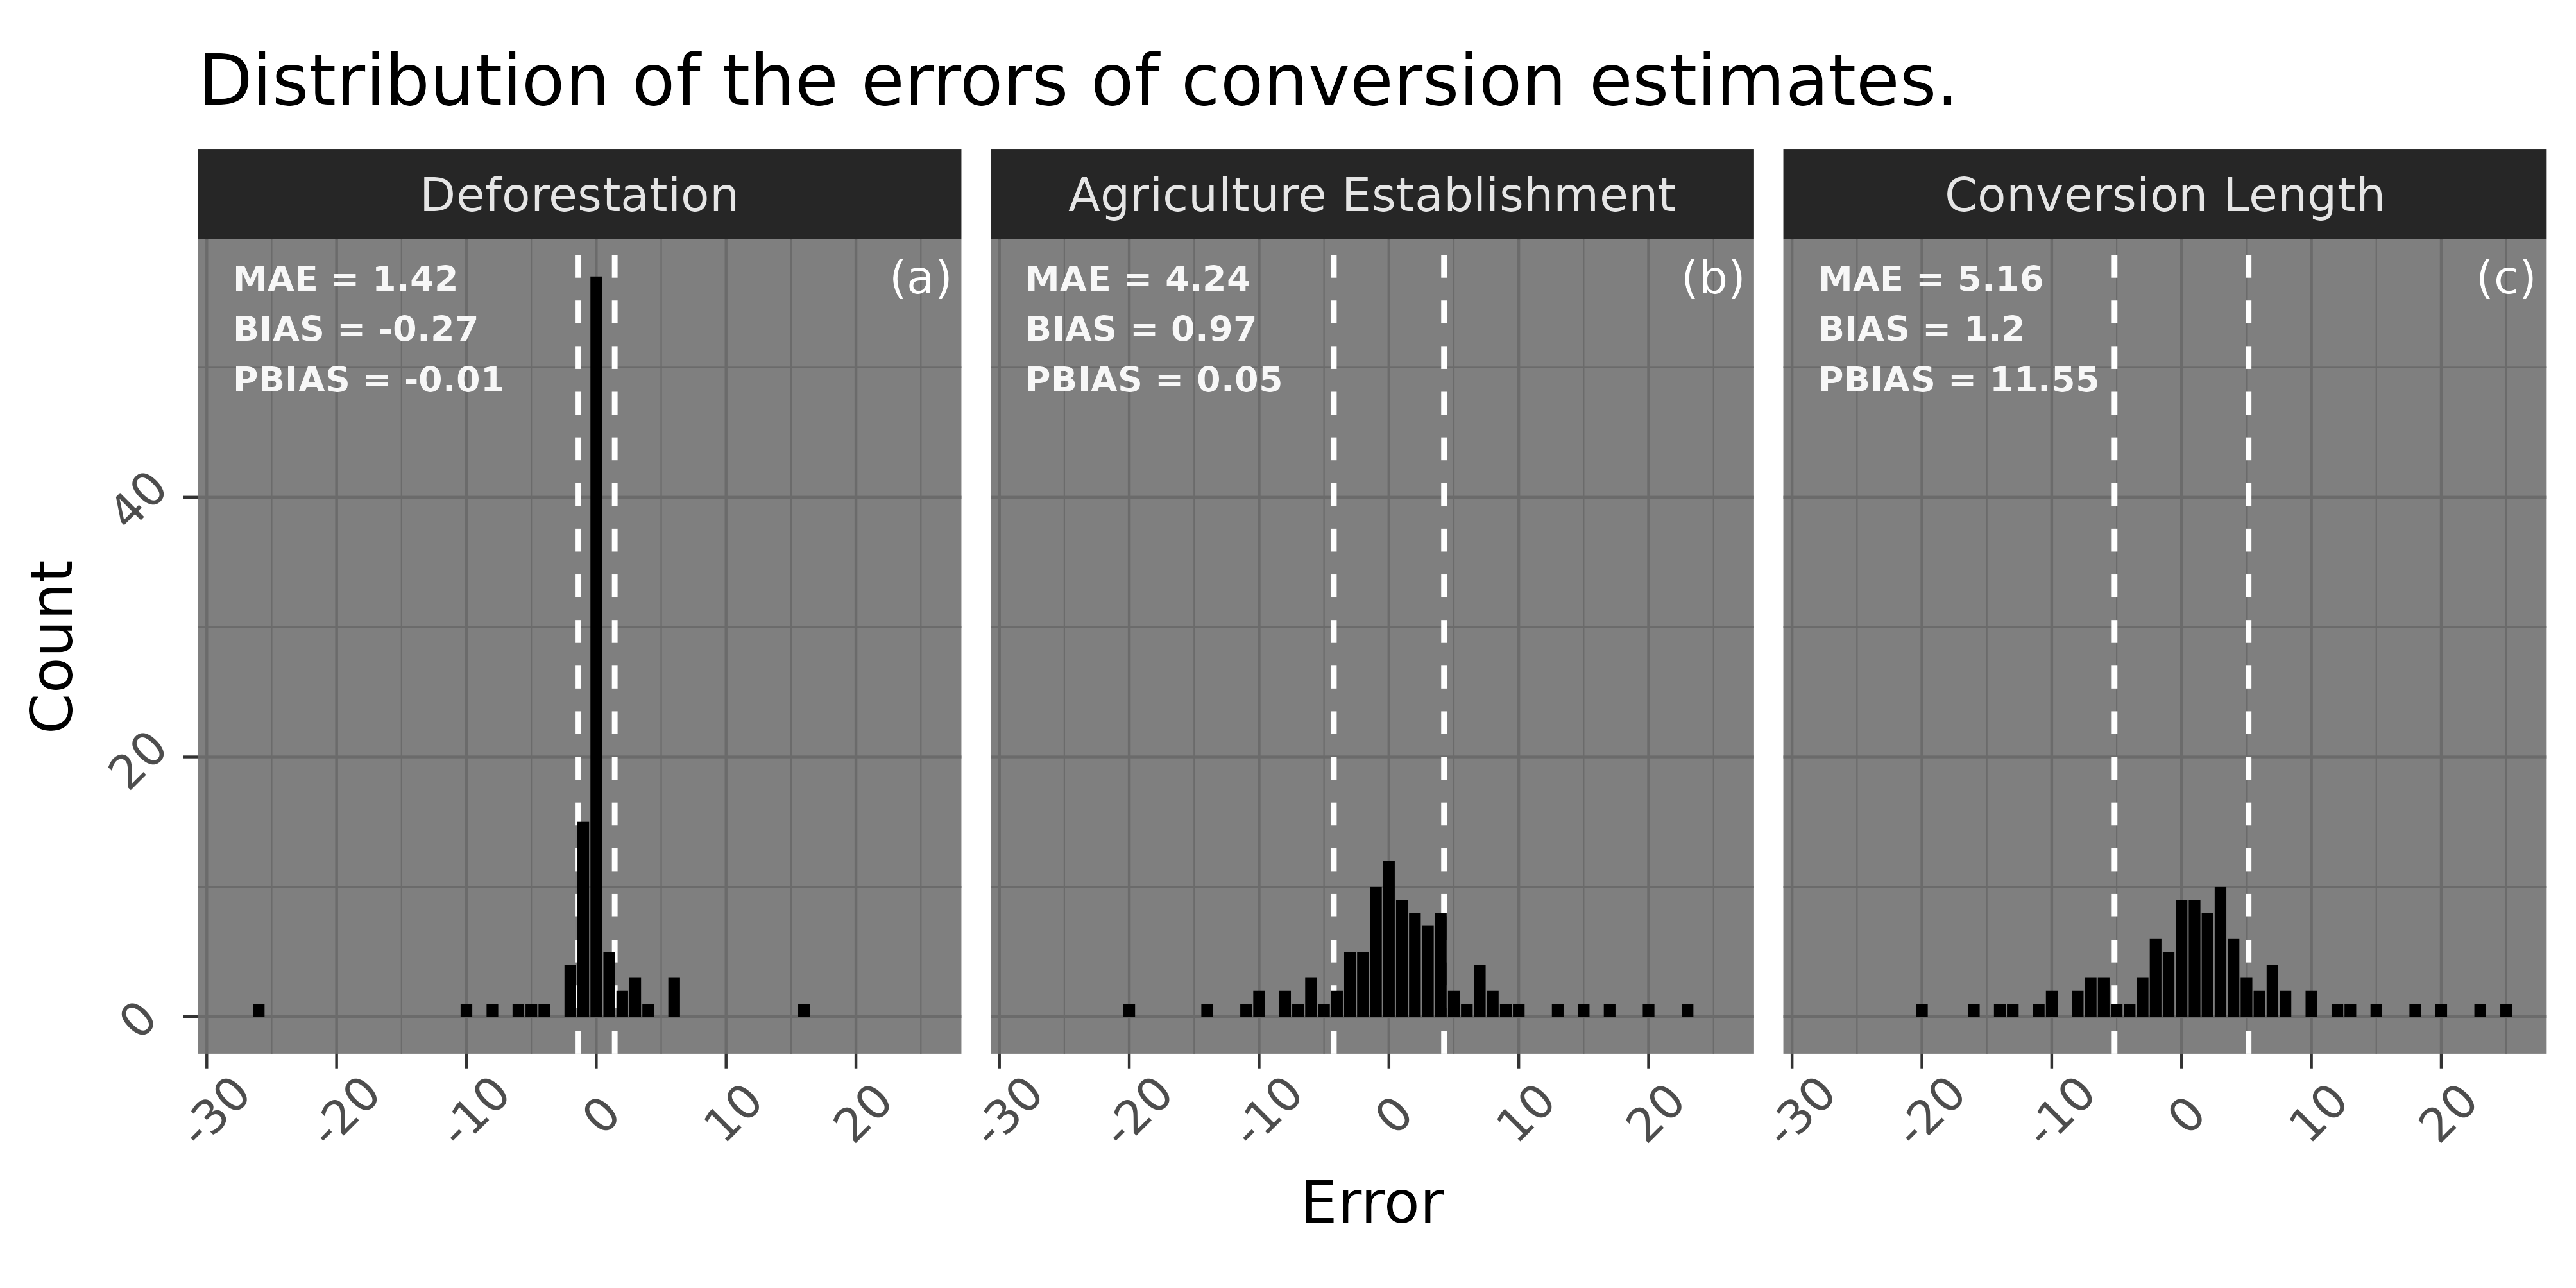
\includegraphics[width=17cm]{figs/error_bars} \caption{ }\label{fig:errorbar-plot}
\end{figure}

\begin{figure}[ht]
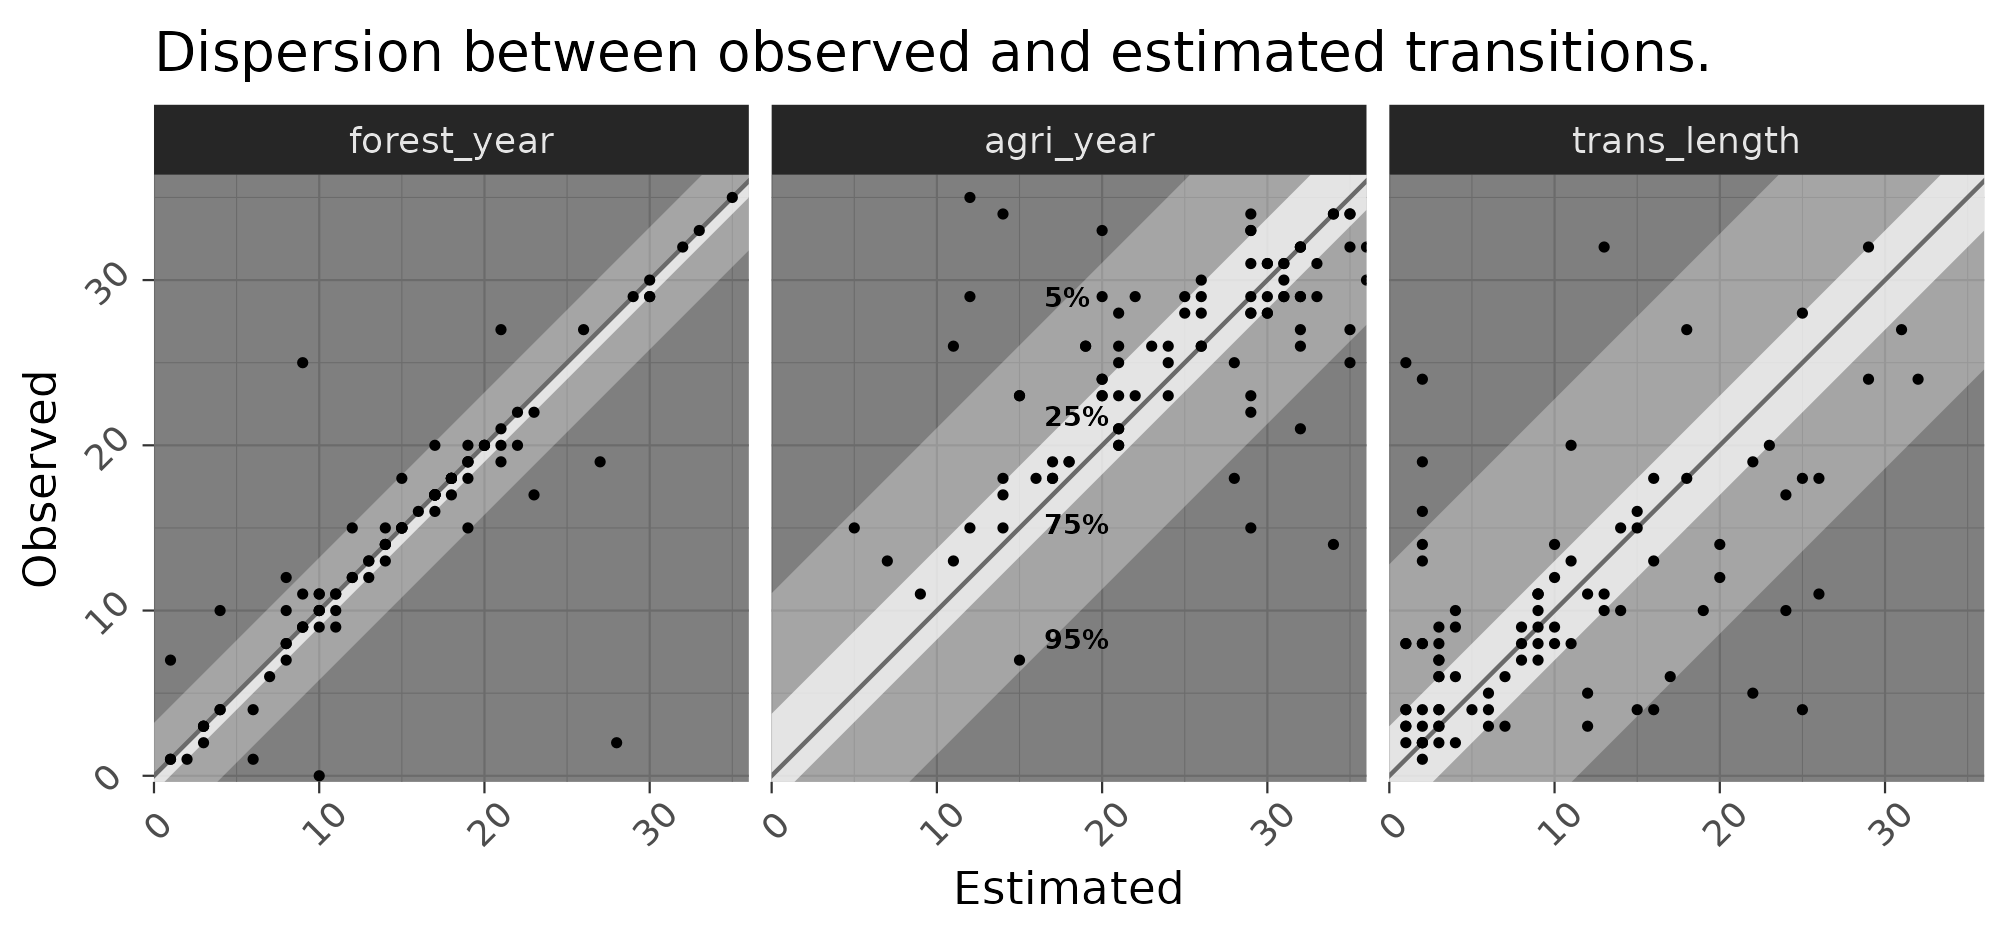
\includegraphics[width=17cm]{figs/error_scatter} \caption{ }\label{fig:errorscatter-plot}
\end{figure}

\subsection{Qualitative assessment}

\conclusions[Conclusions]






%%%%%%%%%%%%%%%%%%%%%%%%%%%%%%%%%%%%%%%%%%
%% optional

%%%%%%%%%%%%%%%%%%%%%%%%%%%%%%%%%%%%%%%%%%

%%%%%%%%%%%%%%%%%%%%%%%%%%%%%%%%%%%%%%%%%%

%%%%%%%%%%%%%%%%%%%%%%%%%%%%%%%%%%%%%%%%%%
\competinginterests{The authors declare no competing interests.} %% this section is mandatory even if you declare that no competing interests are present

%%%%%%%%%%%%%%%%%%%%%%%%%%%%%%%%%%%%%%%%%%

%%%%%%%%%%%%%%%%%%%%%%%%%%%%%%%%%%%%%%%%%%

%% REFERENCES
%% DN: pre-configured to BibTeX for rticles

%% The reference list is compiled as follows:
%%
%% \begin{thebibliography}{}
%%
%% \bibitem[AUTHOR(YEAR)]{LABEL1}
%% REFERENCE 1
%%
%% \bibitem[AUTHOR(YEAR)]{LABEL2}
%% REFERENCE 2
%%
%% \end{thebibliography}

%% Since the Copernicus LaTeX package includes the BibTeX style file copernicus.bst,
%% authors experienced with BibTeX only have to include the following two lines:
%%
\bibliographystyle{copernicus}
\bibliography{references.bib}
%%
%% URLs and DOIs can be entered in your BibTeX file as:
%%
%% URL = {http://www.xyz.org/~jones/idx_g.htm}
%% DOI = {10.5194/xyz}


%% LITERATURE CITATIONS
%%
%% command                        & example result
%% \citet{jones90}|               & Jones et al. (1990)
%% \citep{jones90}|               & (Jones et al., 1990)
%% \citep{jones90,jones93}|       & (Jones et al., 1990, 1993)
%% \citep[p.~32]{jones90}|        & (Jones et al., 1990, p.~32)
%% \citep[e.g.,][]{jones90}|      & (e.g., Jones et al., 1990)
%% \citep[e.g.,][p.~32]{jones90}| & (e.g., Jones et al., 1990, p.~32)
%% \citeauthor{jones90}|          & Jones et al.
%% \citeyear{jones90}|            & 1990


\end{document}
